\documentclass[9pt]{beamer}

\geometry{paperwidth=213.3mm,paperheight=120mm}

\usetheme[{titleformat plain}=smallcaps,
           titleformat title=smallcaps,
           titleformat subtitle=regular,
           titleformat section=smallcaps,
           titleformat frame=smallcaps,
           % numbering=fraction,
          ]{metropolis}
% \usepackage{appendixnumberbeamer}

\definecolor{mLightGreen}{HTML}{14B03D}
\definecolor{vpGreen}{HTML}{66c2a5}
\definecolor{vpOrange}{HTML}{fc8d62}
\providecommand{\iRef}[1]{{\color{mLightGreen}\small $[$#1$]$}}

\usepackage{booktabs}
\usepackage[scale=2]{ccicons}

\usepackage{../_style/common}
\usepackage{../_style/defs}

\usepackage{tikz}
\usetikzlibrary{shapes,arrows}
\usepackage{amsmath, bm}
\usepackage{siunitx}
\usepackage{physics,hepnames}
\usepackage{mathtools}
\usepackage{enumitem}
\setenumerate[1]{%
      label=\protect\usebeamerfont{enumerate item}%
      \protect\usebeamercolor[fg]{enumerate item}%
      \insertenumlabel.}
\setitemize{label=\usebeamerfont*{itemize item}%
    \usebeamercolor[fg]{itemize item}
      \usebeamertemplate{itemize item}}

\usepackage{subfig}
\usepackage{colortbl}
\usepackage{multirow}
\usepackage{pifont}
\usepackage[many]{tcolorbox}

\tcbset{ 
    enhanced,
    size=title,
    sharpish corners, 
    boxrule=0mm, 
    colback=white, 
    % leftrule=2mm,
    % lifted shadow={0.5mm}{-1mm}{4mm}{0.3mm}{black}
    fuzzy shadow={0.5mm}{-1mm}{0mm}{0.3mm}{black}
}

\usepackage{pgfplots}
\usepgfplotslibrary{dateplot}

\usepackage{ulem}

\graphicspath{{pictures/}{../_pictures/}{../2022-Gargnano/pictures/}}

\title{Parton Distribution Functions}
\subtitle{solving the probabilistic inverse problem}
\date{August, 2022}
\author{Alessandro Candido}
%\institute{N3PDF}
\titlegraphic{
    \raisebox{10pt}[0pt][0pt]{
\includegraphics[width=2.5cm]{../_logos/nnpdf_logo.pdf}}\hspace*{10pt}
    \hfill
    \raisebox{5pt}[0pt][0pt]{
\includegraphics[height=0.8cm]{../_logos/n3pdf_logo.pdf}}\hspace*{10pt}
    
\includegraphics[height=1.3cm]{../_logos/erc_logo1.png}

    \vfill\vspace*{230pt}
    
\includegraphics[height=1cm]{../_logos/unimi_logo.png}\hfill
    
\includegraphics[height=1cm]{../_logos/infn_logo.png}\\
    \vspace*{5pt}
    {
        \fontsize{3pt}{3.5pt}\selectfont
        \begin{center}
            This project has received funding from the European Union's Horizon
            2020 research and innovation programme under grant agreement No
            740006\quad 
\includegraphics[height=5pt]{../_logos/eu-flag.jpg}
        \end{center}
    }
}

\begin{document}

\maketitle

\setlist[description]{font=\quad\normalfont\bfseries\scshape\space}
\metroset{block=fill}

\section{The Physics}

\begin{frame}{Theoretical Picture of a Collision}
    \begin{columns}
        \begin{column}{0.5\textwidth}
            Usual picture with 
        \end{column}
        \begin{column}{0.5\textwidth}
            \begin{tcolorbox}[size=tight,sharpish corners,boxrule=0mm]
                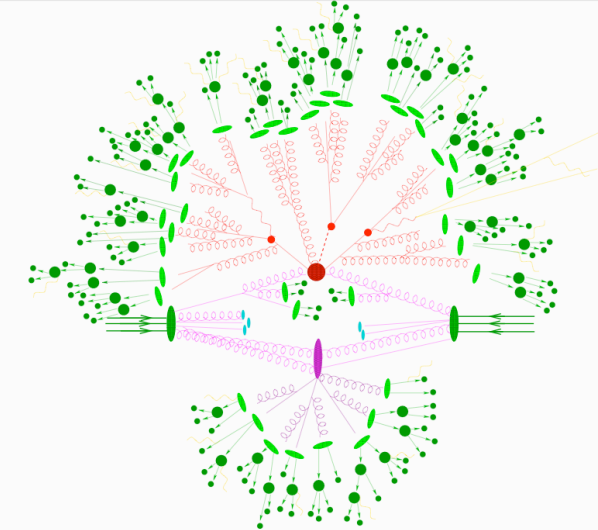
\includegraphics[width=\textwidth]{proton-to-detector}
            \end{tcolorbox}
        \end{column}
    \end{columns}
\end{frame}

\begin{frame}{Soft to Hard Physics}
    \begin{columns}
        \begin{column}{0.5\textwidth}
            Matrix element picture.
        \end{column}
        \begin{column}{0.5\textwidth}
            QCD non perturbative at low energies.
        \end{column}
    \end{columns}
\end{frame}

\begin{frame}{Function space}
    \begin{columns}
        \begin{column}{0.5\textwidth}
            The PDF object: a set of functions (one per flavor) $f_i: [0, 1] \to \mathbb{R}$
        \end{column}
        \begin{column}{0.5\textwidth}
            \begin{tcolorbox}
                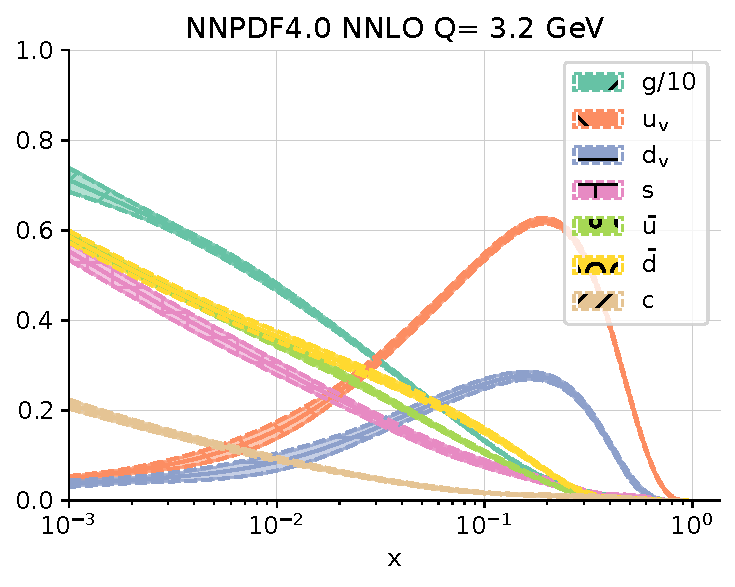
\includegraphics[width=\textwidth]{pdfs_pdg_Qs0_plot_flavours}
            \end{tcolorbox}
        \end{column}
    \end{columns}
\end{frame}

\section{Inverse Problem}

\begin{frame}{Direct problem}
    Luigi's Tikz diagram, hand drawn.
\end{frame}

\begin{frame}{FK tables}
    Which is the map?
    Just to give the idea of what I'm working on, and that is all but trivial.

    Linear and quadratic map, plus composite (few examples).
\end{frame}

\begin{frame}{Function space}
    \begin{columns}
        \begin{column}{0.5\textwidth}
            A function $f: \mathbb{R} \to \mathbb{R}$ (or suitable intervals)
            lives in an infinite-dimensional space.
            \vspace*{20pt}

            This has a simple consequence:
            \begin{block}{Under-determination}
                Fitting an \textbf{unknown function} on a finite number of data
                is always an \textbf{under-determined} problem.
            \end{block}
            \vspace*{20pt}

            How to choose a solution, when \alert{many} are available and
            \alert{equivalent}?
        \end{column}
        \begin{column}{0.5\textwidth}
            \begin{figure}
                \centering
                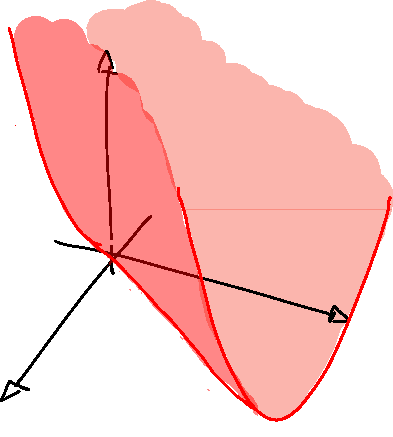
\includegraphics[width=0.6\textwidth]{underdetermined}
                \caption{Possible $\chi^2$ profile in 2D parameter space.}
            \end{figure}
        \end{column}
    \end{columns}
\end{frame}

\begin{frame}{Solutions in the Assumptions}
    \vspace*{10pt}
    \begin{center}
        There are two main ways to attack the problem.
    \end{center}
    \vspace*{10pt}

    \begin{columns}
        \begin{column}{0.5\textwidth}
            1. One consists in \textit{reducing the number of parameters}, by
            \textbf{slicing} a suitable \textbf{hyperplane}.
            \footnote{Not containing zero-directions.}
            \vspace*{10pt}

            This is what we do in PDFs when choosing a \alert{\textbf{fixed
            parametrization}}: we decide which parameters to fit, and take a
            single given value for everything else.
            \vspace*{10pt}

            \begin{figure}
                \centering
                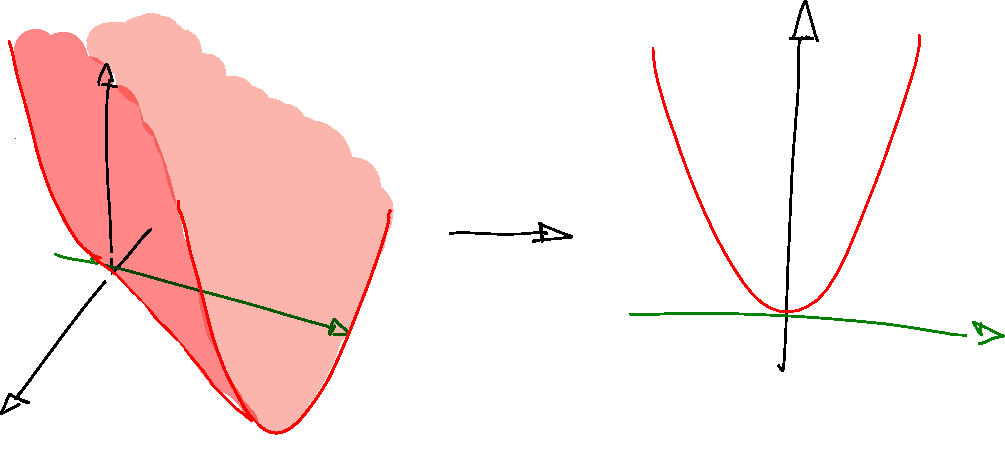
\includegraphics[width=0.8\textwidth]{sliced}
                \caption{$\chi^2$ profile in sliced parameter space.}
            \end{figure}
            \vspace*{10pt}
        \end{column}
        \begin{column}{0.5\textwidth}
            2. The second approach removes the zero-direction by adding
            \textbf{regularization}.
            \vspace*{10pt}

            This is what the \alert{\textbf{Neural Network}} (and its training
            algorithm) is doing under the hood.
            \vspace*{10pt}

            \begin{figure}
                \centering
                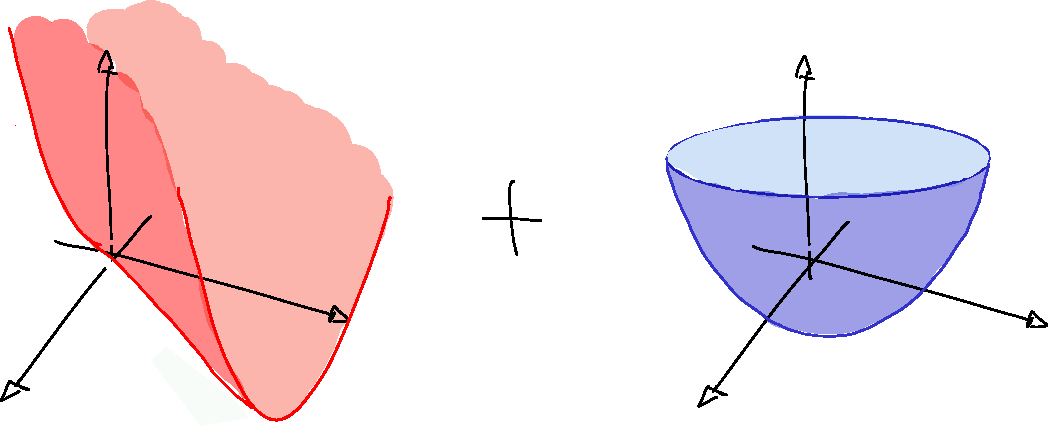
\includegraphics[width=0.8\textwidth]{regularized}
                \caption{$\chi^2$ profile plus regularization function.}
            \end{figure}
        \end{column}
    \end{columns}
\end{frame}

\begin{frame}{So Which?}
    \vspace*{30pt}
    \begin{columns}
        \begin{column}{0.5\textwidth}
            Then which one should we choose?
            \vspace*{10pt}

            \begin{figure}
                \centering
                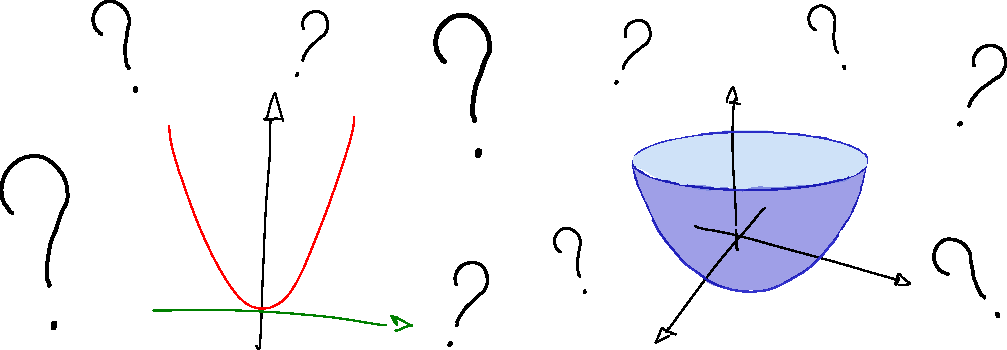
\includegraphics[width=0.9\textwidth]{choice}
            \end{figure}

            \vspace*{10pt}
            There is \textbf{not} an \alert{\textbf{absolute best answer}},
            because both procedures might be \textit{\textbf{arbitrary}}.
        \end{column}
        \begin{column}{0.5\textwidth}
            So, we need a guiding principle to make a good choice, and a good one is:
            \begin{center}
                \itshape
                \bfseries
                Choices should encode physics assumptions
            \end{center}
            and as little arbitrariness as possible\footnote{
                Though nothing is actually bias-free, so better to know and
                declare your bias, rather than hiding it.
            }.

            \vspace*{20pt}
            So what about PDFs?
            \begin{description}
                \item[cuts] cutting the space (fixed parametrization) is no
                    bad, \textbf{if you know how to do it}: you need
                    \alert{\textbf{precise theoretical insight}} on the
                    \alert{\textbf{\pdf shape}}
                \item[regularization] also this need as much motivation as the
                    former, but it makes \textit{to shift the focus} from the
                    exact shape to more abstract \alert{\textbf{features}}
            \end{description}
            \vspace*{20pt}
        \end{column}
    \end{columns}
\end{frame}

\section{Uncertainties = Distribution}

\begin{frame}{Propagating Error}
    Hessian Approach
\end{frame}

\begin{frame}{Replicas}
    \nnpdf{} Approach

    Na\"ive idea: the error comes from data, let's propagate the data
    distribution back through the \textit{inverse function}:
    \begin{equation*}
        \mathcal{F}(D) = \argmin_\theta\left(\mathcal{L}(D)\right)
    \end{equation*}
\end{frame}

\begin{frame}{The NN}
    \begin{center}
        What is then doing the neural network (NN)? Why is it working so well?
    \end{center}
    \vspace*{10pt}

    \begin{columns}
        \begin{column}{0.5\textwidth}
            \begin{figure}
                \centering
                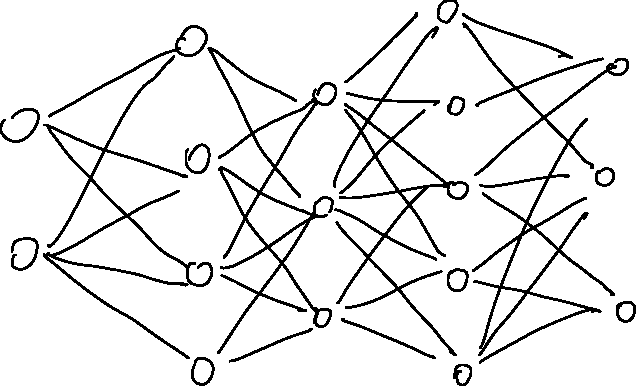
\includegraphics[width=0.6\textwidth]{nn}
            \end{figure}

            \vspace*{10pt}
                Essentially, the \textit{NN is encoding} an
                \alert{\textbf{interpolation hypothesis}} \textit{in the
                architecture \textbf{and} training algorithm}.
        \end{column}
        \begin{column}{0.5\textwidth}
            While both the approaches are limiting \textit{model complexity},
            the \textbf{Neural Network} is free enough to follow strong
            \textbf{data trends}.

            \vspace*{10pt}
            \begin{exampleblock}{Physical Wiggles}
                A criticism we collected has been about \textit{NN opaque
                assumptions} might \textbf{prevent} to follow \textbf{small
                physical fluctuations}, but it is actually the other way
                round:\footnote{In principle, yet to be proven in practice.}

                \begin{description}
                    \item[fixed param.] in this case, you can only find
                        oscillations you are allowing for, so you need to know
                        in advance \textbf{each and every wiggle} to
                        discriminate physical ones from noise
                    \item[NN] all wiggles are deweighted, but physical wiggles
                        should be resolved more and more by data, so
                        \textit{"enough precision"} in the
                        \alert{\textbf{data}} will naturally
                        \textbf{\alert{overwhelm} the theoretical
                        \alert{(learning) bias}}
                \end{description}
            \end{exampleblock}
        \end{column}
    \end{columns}
\end{frame}

\begin{frame}{Propagating Error}
    \nnpdf{} Approach - reinterpreted
    \let\thefootnote\relax\footnotetext{
        \paperref{https://doi.org/10.1140/epjc/s10052-022-10297-x}{\textit{L. Del
        Debbio, T. Giani, M. Wilson}, Eur.Phys.J.C 82 (2022) 4, 330}
    }. (Luigi's paper)

    Hints for a better approach (if it's equivalent to something meaningful,
    maybe it would be worth to try that something).

    
\end{frame}

\section{Trust the Results}

\begin{frame}{Dataset}
    Variety of datasets, to cover different features of the underlying object.
    
    \begin{center}
        \begin{tcolorbox}[width=0.7\textwidth]
            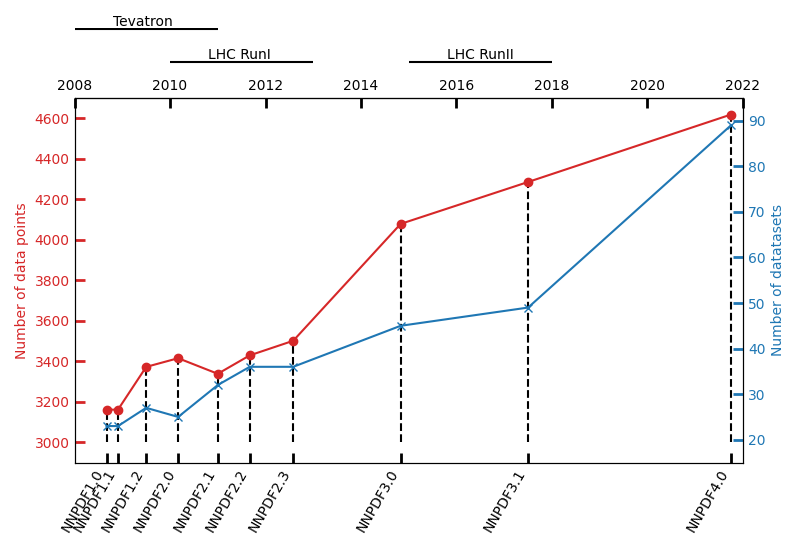
\includegraphics[width=\textwidth]{data}
        \end{tcolorbox}
    \end{center}
\end{frame}

\begin{frame}{Amazing Black Box}
    \begin{columns}
        \begin{column}{0.5\textwidth}
            Common criticism is the NN being a black box
        \end{column}
        \begin{column}{0.5\textwidth}
            Shiny Black box picture
        \end{column}
    \end{columns}
\end{frame}

\begin{frame}{Closure Tests}
    Controls data region.

    \begin{itemize}
        \item Level 0, $\chi^2_{expected} \sim 0$
        \item Level 1, $\chi^2_{expected} \sim 1$
        \item Level 2, $\chi^2_{expected} \sim 2$
    \end{itemize}
\end{frame}

\begin{frame}{Future Tests}
    Controls extrapolation region.
\end{frame}

\section{Results}

\begin{frame}{Uncertainties - Data Region}
    \begin{columns}
        \begin{column}{0.5\textwidth}
            Ciao
        \end{column}
        \begin{column}{0.5\textwidth}
            \begin{tcolorbox}
                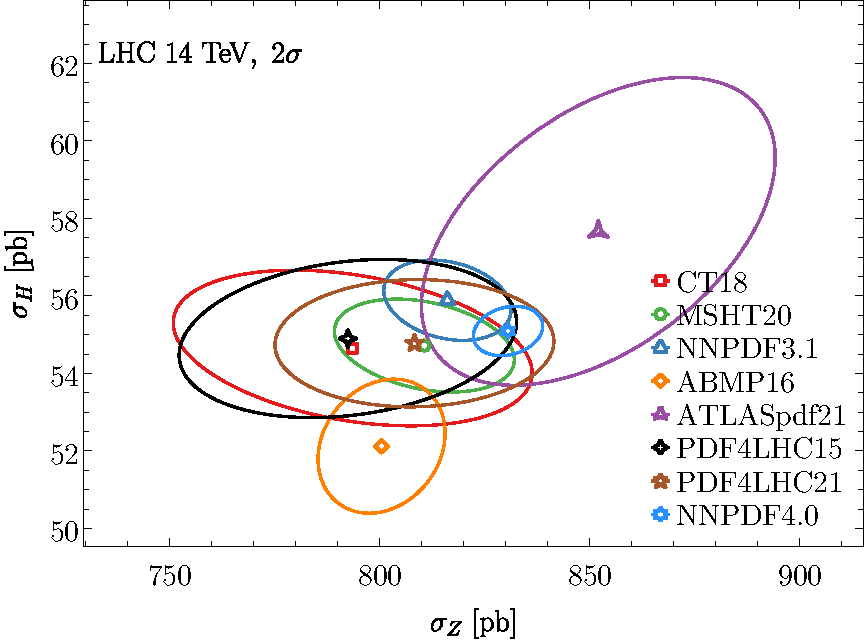
\includegraphics[width=\textwidth]{Corr_Z2H14TeV_2sigma}
            \end{tcolorbox}
        \end{column}
    \end{columns}
\end{frame}

\begin{frame}{Uncertainties - Extrapolation - Large $x$}
    \begin{columns}
        \begin{column}{0.5\textwidth}
            \begin{tcolorbox}[size=small,sharpish corners,boxrule=0mm]
                \centering
                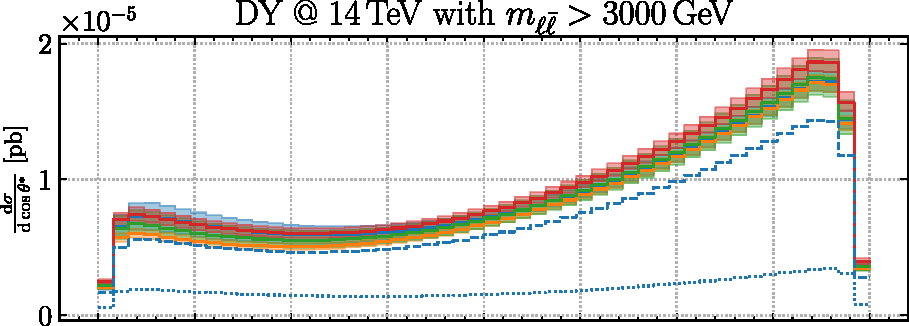
\includegraphics[width=0.49\textwidth]{NNPDF_DY_14TEV_BSM_AFB_COS_3000}
                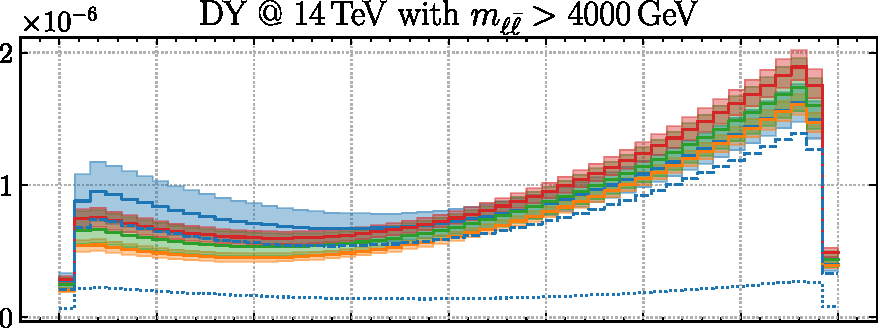
\includegraphics[width=0.49\textwidth]{NNPDF_DY_14TEV_BSM_AFB_COS_4000}
            \end{tcolorbox}

            \vspace*{20pt}
            Result already partially encoded in the hypothesis.
            \vspace*{20pt}

            \begin{tcolorbox}[size=small,sharpish corners,boxrule=0mm]
                \centering
                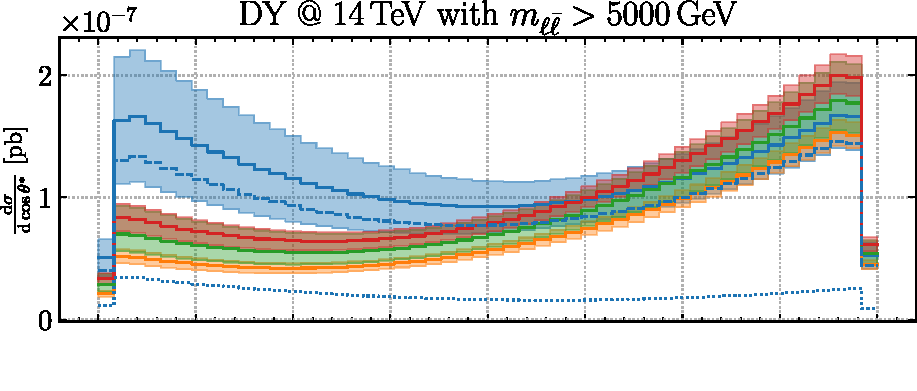
\includegraphics[width=0.49\textwidth]{NNPDF_DY_14TEV_BSM_AFB_COS_5000}
                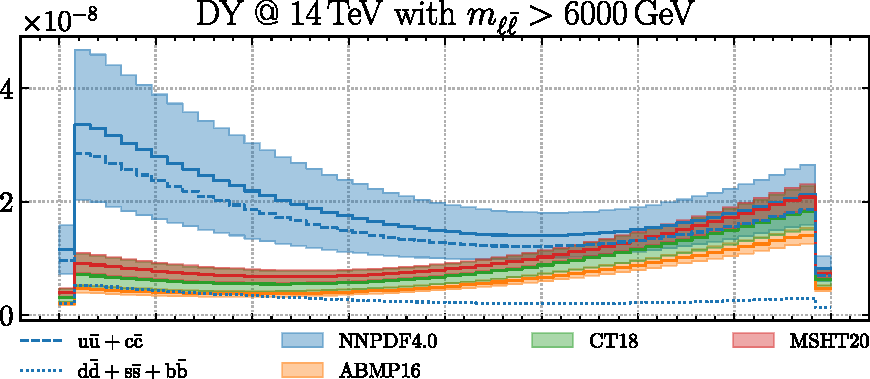
\includegraphics[width=0.49\textwidth]{NNPDF_DY_14TEV_BSM_AFB_COS_6000}
            \end{tcolorbox}
        \end{column}
        \begin{column}{0.5\textwidth}
            \begin{tcolorbox}
                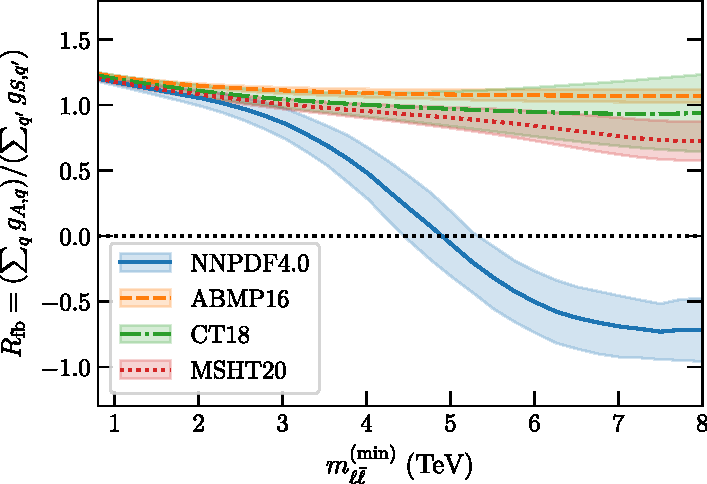
\includegraphics[width=\textwidth]{asym_coeff_mlldep}
            \end{tcolorbox}
        \end{column}
    \end{columns}
\end{frame}

\begin{frame}{Intrinsic Charm}
    \begin{columns}
        \begin{column}{0.5\textwidth}
            \begin{tcolorbox}
                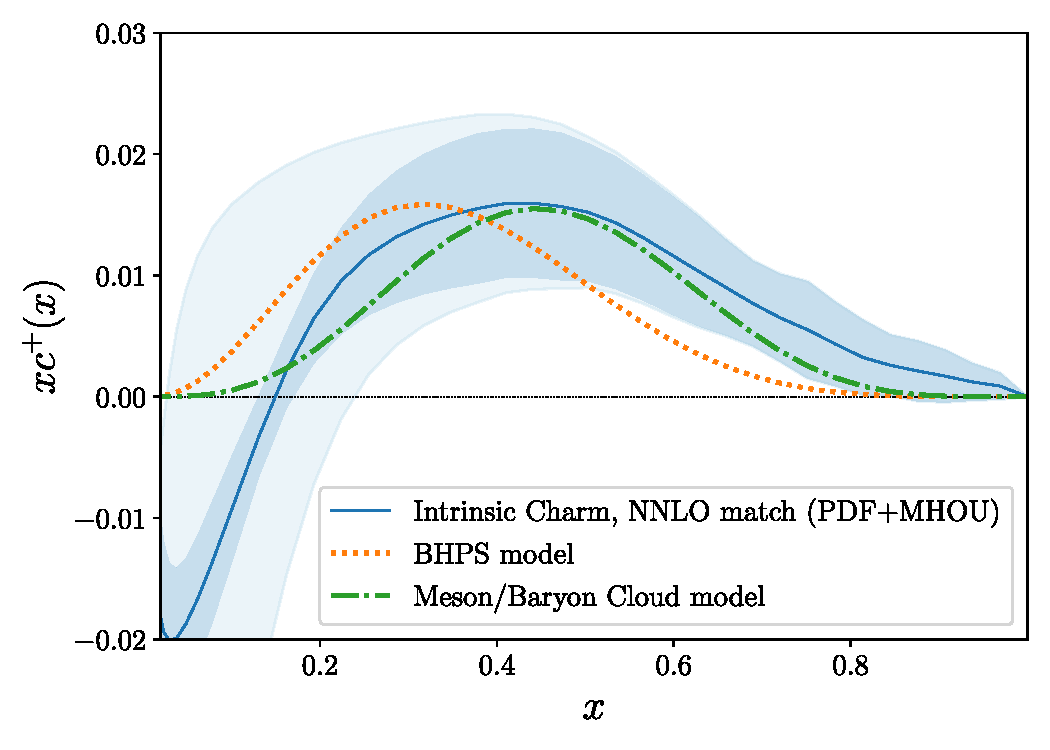
\includegraphics[width=\textwidth]{nf3_to_models}
            \end{tcolorbox}
        \end{column}
        \begin{column}{0.5\textwidth}
            \begin{tcolorbox}
                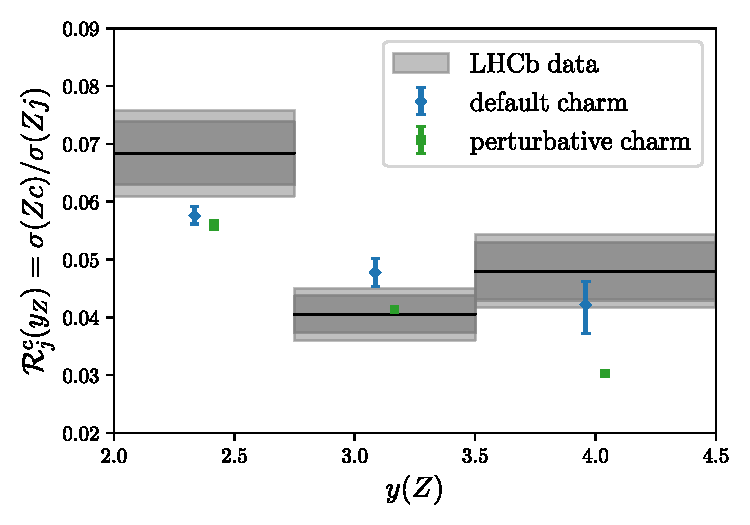
\includegraphics[width=\textwidth]{lhcb-zcharm-pheno}
            \end{tcolorbox}
        \end{column}
    \end{columns}
\end{frame}

\section{Conclusions}

\begin{frame}{Summary}
\end{frame}

\begin{frame}{Tools and References}
    \begin{columns}
        \begin{column}{0.5\textwidth}
            For all info about the collaboration:

            \url{https://nnpdf.mi.infn.it}
        \end{column}
        \begin{column}{0.5\textwidth}
            \paperref{https://doi.org/10.1140/epjc/s10052-021-09747-9}{Eur.Phys.J.C 81 (2021) 10, 958}

            \githuburl{https://github.com/NNPDF/nnpdf}

            \url{https://docs.nnpdf.science}

            \begin{figure}
                \centering
                
\includegraphics[width=0.15\textwidth]{tensorflow}
                \hspace*{0.25\textwidth}
                
\includegraphics[width=0.15\textwidth]{python}
            \end{figure}
        \end{column}
    \end{columns}
\end{frame}

\begin{frame}[standout]
    Thanks for your attention!
\end{frame}

\appendix

\begin{frame}{Looking for Insights}
    \begin{columns}
        \begin{column}{0.5\textwidth}
            \textit{NNPDF "framework"} is much \textbf{\textit{more}} than a Neural
            Network only:
            \begin{itemize}
                \item nice representation of a generic distribution (\textbf{replicas})
                \item many \textbf{tests} in place
                \item \textbf{fast theory} framework
                \item \textbf{lots of data} implemented
                \begin{itemize}
                    \item both theory calculation and
                    \item commondata implementation with uncertainties
                        (including correlated systematics)
                \end{itemize}
                \item and more\dots
            \end{itemize}
            \vspace*{10pt}

            \begin{center}
                \itshape
                We do \textbf{not} want to \textbf{loose} \alert{\textbf{any}} of these.
            \end{center}
        \end{column}
        \begin{column}{0.5\textwidth}
            But sometimes we \textbf{lack insight}: we have tests for this, but
            they are not always a handy tool to answer all questions.
            \vspace*{10pt}

            \begin{exampleblock}{Hopscotch}
                \begin{center}
                    \itshape
                    What are our criticism to CT replicas?
                \end{center}
                Mostly we blame the method, but little criticism on the result.

                Some \textbf{physical assumptions} have been checked:
                \begin{itemize}
                    \item $\chi^2$ vs $\chi^2_{t_0}$
                    \item integrability and sum rules
                    \item positivity
                \end{itemize}

                But it might be hidden in the NN \textbf{regularization}.
            \end{exampleblock}

        \end{column}
    \end{columns}

    \vspace*{10pt}
    Another limitation\footnote{
        Actually, this is where everything started from.
    } is that the current methodology need to make a \textbf{fit to \alert{one
    sample} at a time}. The distribution is only the result of many fits.

    \vspace*{-5pt}
    \begin{center}
        \itshape
        \bfseries
        What if we could fit the distribution all at once?
    \end{center}
    \vspace*{-10pt}
\end{frame}

\begin{frame}{Restart from Bayes}
    \begin{columns}
        \begin{column}{0.5\textwidth}
            Typical examples of ML are:
            \begin{itemize}
                \item image and speech recognition
                \item generative tasks,
                \item style transfer
                \item and so on...
            \end{itemize}
            \vspace*{10pt}

            All these problems have in common:
            \begin{center}
                very \textbf{high dimensional} objects, with
                \alert{\textbf{poor analytical/algorithmic insight}} on its
                structure.   
            \end{center}
            Working out an explicit and effective representation for them would
            be difficult.
            \vspace*{10pt}

            Not the case for \pdf{}s: \textbf{math language description} and
            \textbf{clear analytic properties} at hand (sum rules, power-like
            behavior, and so on\dots).
        \end{column}
        \begin{column}{0.5\textwidth}
            \begin{figure}
                \centering
                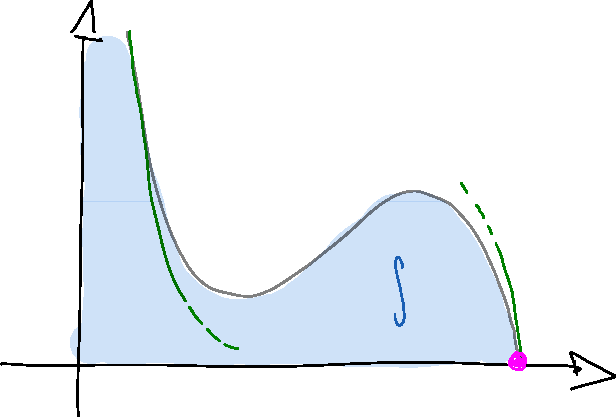
\includegraphics[width=0.6\textwidth]{pdf}
                \caption{\pdf analytical features.}
            \end{figure}

            Then, we can follow a rather simple analytical approach:
            \begin{equation*}
                P(A|B) = \frac{P(B|A) P(A)}{P(B)}
            \end{equation*}
            
            Bayes formula exposes \textbf{regularization} explicitly in the
            prior, so the assumptions are analytically transparent.
        \end{column}
    \end{columns}
\end{frame}

\begin{frame}{Prior Choice \& Implementation}
    \begin{center}
        But then the question: \textbf{\textit{which prior?}}
    \end{center}
    \begin{columns}
        \begin{column}{0.5\textwidth}
            \textbf{A:} a Gaussian process
            \begin{figure}
                \centering
                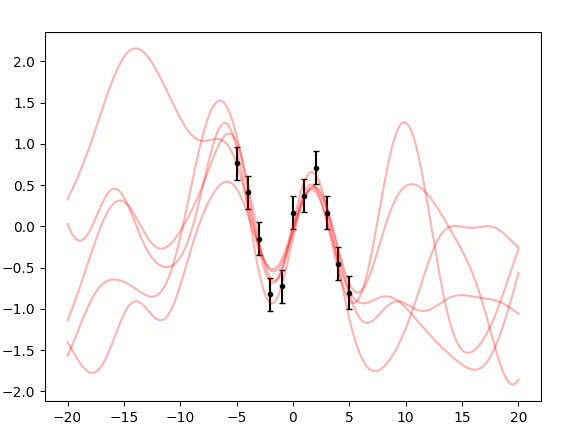
\includegraphics[width=0.9\textwidth]{sine6}
            \end{figure}

            Essentially a \textit{multi-Gaussian} with a \textbf{metric-driven
            kernel}, with the motivation that is simple, and sufficiently
            flexible.
        \end{column}
        \begin{column}{0.5\textwidth}
            Basic ideas:
            \begin{description}
                \item[parametrization] exactly our delivery: we use \pdf values
                    at grid points (we would no expose more degree of freedom
                    anyhow, so no need to use them)
                \item[transformations] data are not in the \pdf space, but we
                    can use linear and non-linear (quadratic) transformations
                \item[sum rules] the Gaussian process allow us to impose them
                    analytically (in practice, it is easier to impose them as
                    \textit{zero-error data}, but it is only a technicality)
                    \begin{itemize}
                        \item the important thing is that we can
                            \textbf{constrain integral and derivatives} as much
                            as the process, thanks to the \textit{metrical
                            kernel}
                    \end{itemize}
                \item[integrability] integrability and extrapolation behavior
                    it is implemented as constraints on hyper-parameters
                \item[positivity] we can implement as constraint on the process
            \end{description}
        \end{column}
    \end{columns}
\end{frame}


\begin{frame}{(Very) Preliminary Results}
    \vspace*{10pt}
    \begin{figure}
        \centering
        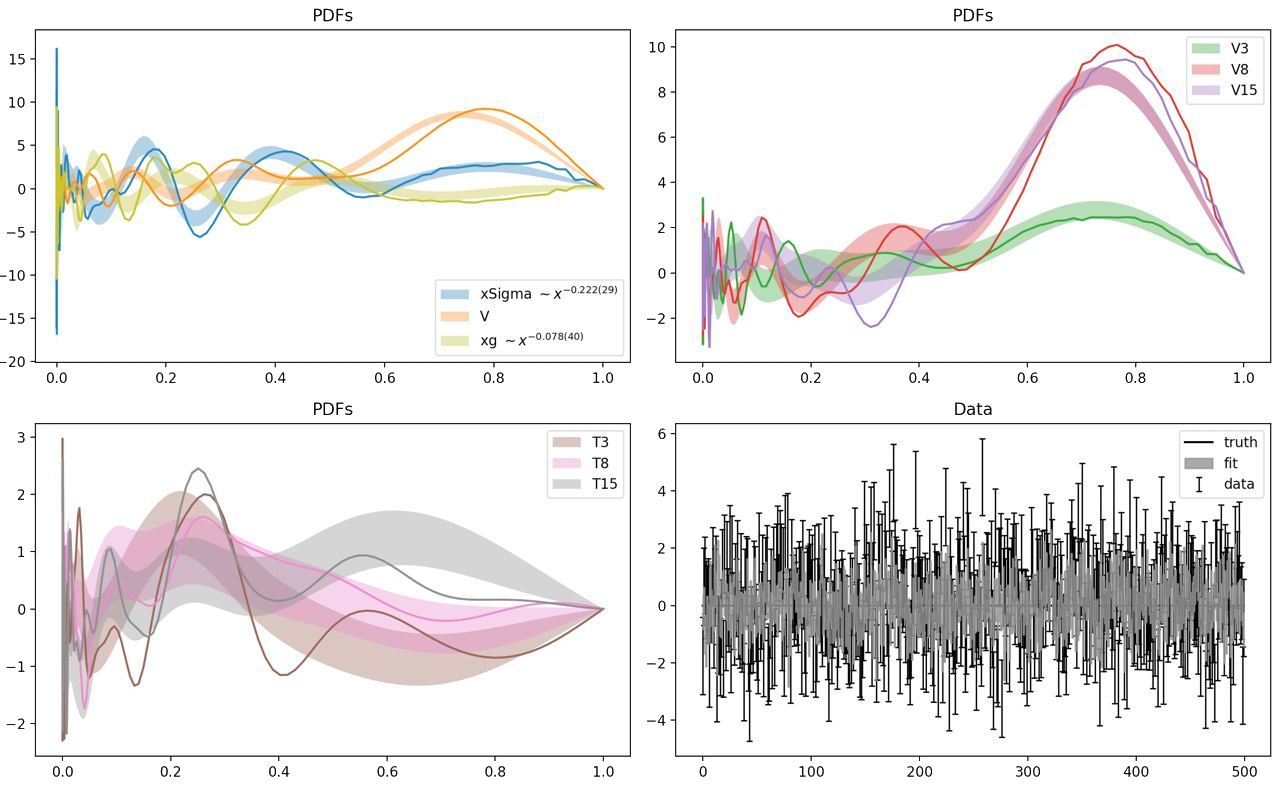
\includegraphics[width=0.75\textwidth]{fit-pdf}
        \caption{
            Even with completely random data and theory, we get a valence like
            structure (\textbf{valence peak}, wrong place, wrong height) by
            virtue of \textbf{sum rules}. Still, they are too much
            unconstrained to get correct values.
        }
    \end{figure}
\end{frame}

\begin{frame}{Hyper-opt}
    You can get the full distribution, including \textbf{hyper-parameters}:
    \begin{equation*}
        P(A|B;\lambda) = \frac{P(B|A) P(A;\lambda)}{P(B)}
    \end{equation*}

    And, \textit{if you wish}, you can \alert{\textbf{hyper-optimize}} to get a
    single value:
    \begin{equation*}
        \begin{cases}
            \lambda^* = \max_{\lambda \in \Lambda} P(A|B;\lambda)\\
            P(A|B) = \max_{\lambda \in \Lambda} P(A|B;\lambda) = P(A|B; \lambda^*)
        \end{cases}
    \end{equation*}
    
    This is just the \textbf{Maximum A Posteriori (MAP)} estimate on
    hyper-parameters, but the full distribution contains more information.

    But at that point you might want to choose a \textbf{hyper-prior}, that
    will affect also the MAP estimate of hyper-parameters (you decide where to
    stop\dots but essentially is all \textit{part of your prior}).
\end{frame}

\begin{frame}{Further results}
    \vspace*{30pt}
    \begin{columns}
        \begin{column}{0.6\textwidth}
            \begin{figure}
                \centering
                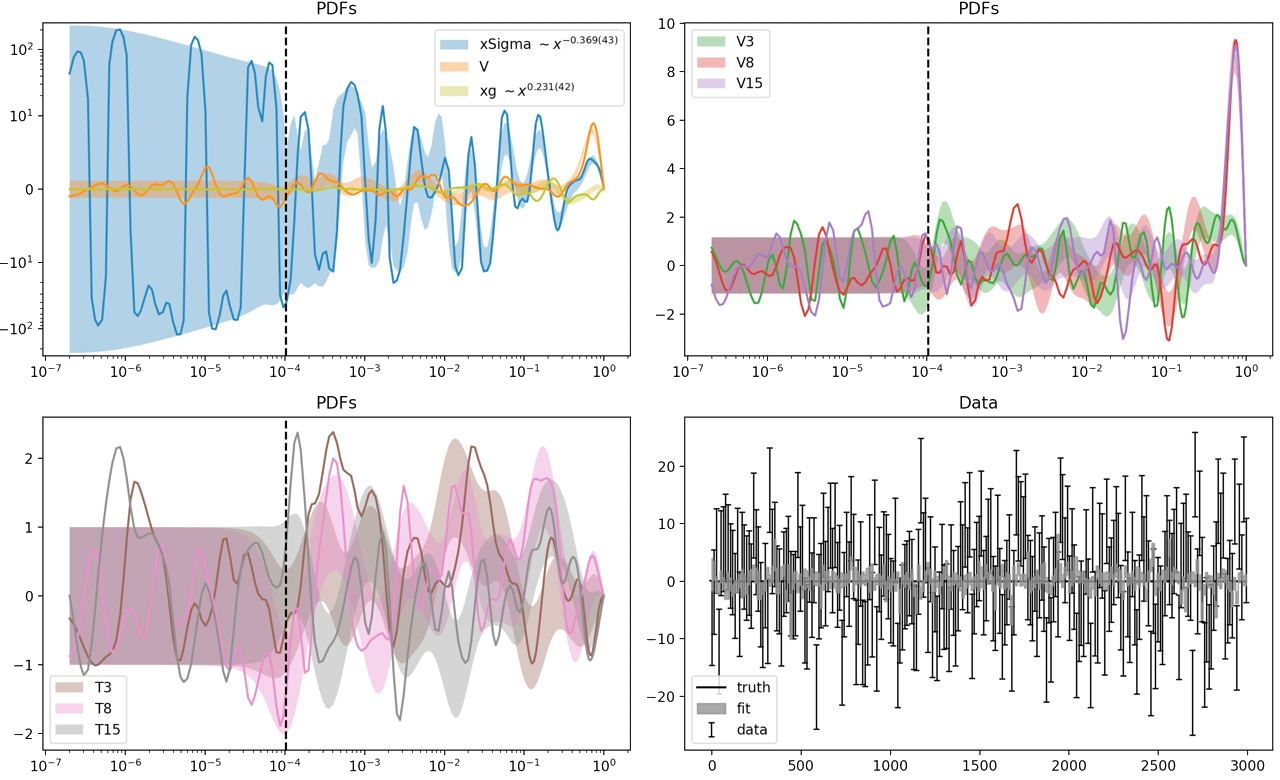
\includegraphics[width=\textwidth]{fit-pdf-new}
                \caption{
                    New fit candidate, with less random data (still pretty
                    random).
                }
            \end{figure} 
        \end{column}
        \begin{column}{0.4\textwidth}
            \begin{figure}
                \centering
                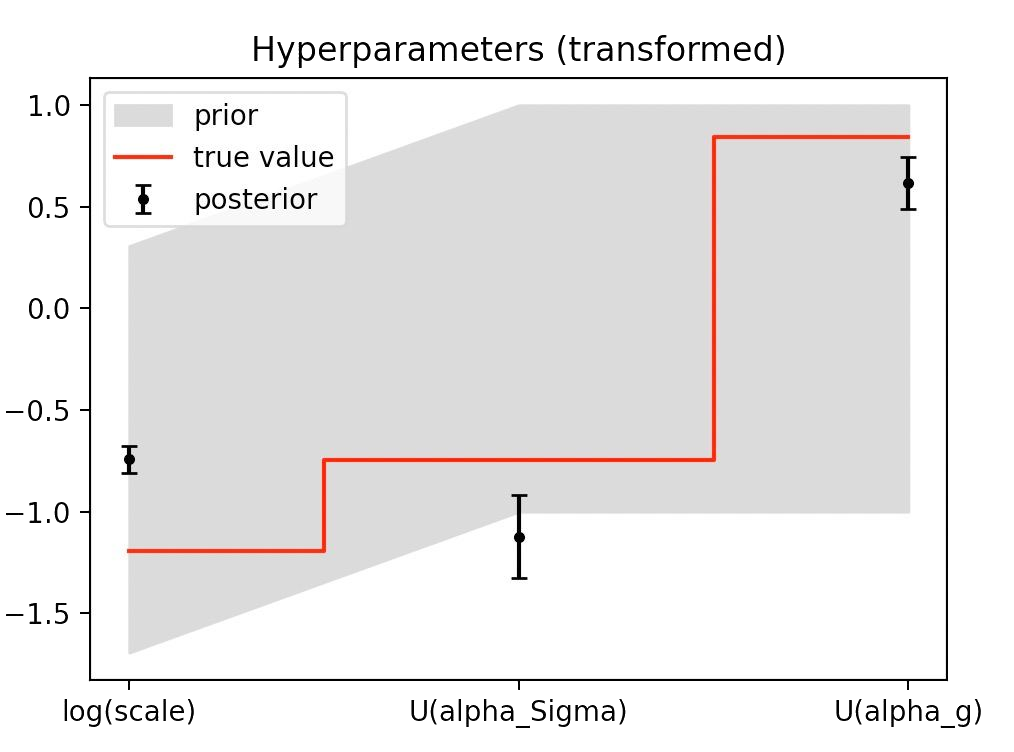
\includegraphics[width=\textwidth]{fit-hyper-new}
                \caption{
                    Hyperparameters fit: notice that while exponents are
                    working, we are still missing the correlation length.
                }
            \end{figure} 
        \end{column}
    \end{columns}
\end{frame}

\end{document}
